% Options for packages loaded elsewhere
\PassOptionsToPackage{unicode}{hyperref}
\PassOptionsToPackage{hyphens}{url}
\PassOptionsToPackage{dvipsnames,svgnames,x11names}{xcolor}
%
\documentclass[
  10pt,
]{article}

\usepackage{amsmath,amssymb}
\usepackage{iftex}
\ifPDFTeX
  \usepackage[T1]{fontenc}
  \usepackage[utf8]{inputenc}
  \usepackage{textcomp} % provide euro and other symbols
\else % if luatex or xetex
  \usepackage{unicode-math}
  \defaultfontfeatures{Scale=MatchLowercase}
  \defaultfontfeatures[\rmfamily]{Ligatures=TeX,Scale=1}
\fi
\usepackage{lmodern}
\ifPDFTeX\else  
    % xetex/luatex font selection
\fi
% Use upquote if available, for straight quotes in verbatim environments
\IfFileExists{upquote.sty}{\usepackage{upquote}}{}
\IfFileExists{microtype.sty}{% use microtype if available
  \usepackage[]{microtype}
  \UseMicrotypeSet[protrusion]{basicmath} % disable protrusion for tt fonts
}{}
\makeatletter
\@ifundefined{KOMAClassName}{% if non-KOMA class
  \IfFileExists{parskip.sty}{%
    \usepackage{parskip}
  }{% else
    \setlength{\parindent}{0pt}
    \setlength{\parskip}{6pt plus 2pt minus 1pt}}
}{% if KOMA class
  \KOMAoptions{parskip=half}}
\makeatother
\usepackage{xcolor}
\setlength{\emergencystretch}{3em} % prevent overfull lines
\setcounter{secnumdepth}{-\maxdimen} % remove section numbering
% Make \paragraph and \subparagraph free-standing
\makeatletter
\ifx\paragraph\undefined\else
  \let\oldparagraph\paragraph
  \renewcommand{\paragraph}{
    \@ifstar
      \xxxParagraphStar
      \xxxParagraphNoStar
  }
  \newcommand{\xxxParagraphStar}[1]{\oldparagraph*{#1}\mbox{}}
  \newcommand{\xxxParagraphNoStar}[1]{\oldparagraph{#1}\mbox{}}
\fi
\ifx\subparagraph\undefined\else
  \let\oldsubparagraph\subparagraph
  \renewcommand{\subparagraph}{
    \@ifstar
      \xxxSubParagraphStar
      \xxxSubParagraphNoStar
  }
  \newcommand{\xxxSubParagraphStar}[1]{\oldsubparagraph*{#1}\mbox{}}
  \newcommand{\xxxSubParagraphNoStar}[1]{\oldsubparagraph{#1}\mbox{}}
\fi
\makeatother

\usepackage{color}
\usepackage{fancyvrb}
\newcommand{\VerbBar}{|}
\newcommand{\VERB}{\Verb[commandchars=\\\{\}]}
\DefineVerbatimEnvironment{Highlighting}{Verbatim}{commandchars=\\\{\}}
% Add ',fontsize=\small' for more characters per line
\usepackage{framed}
\definecolor{shadecolor}{RGB}{241,243,245}
\newenvironment{Shaded}{\begin{snugshade}}{\end{snugshade}}
\newcommand{\AlertTok}[1]{\textcolor[rgb]{0.68,0.00,0.00}{#1}}
\newcommand{\AnnotationTok}[1]{\textcolor[rgb]{0.37,0.37,0.37}{#1}}
\newcommand{\AttributeTok}[1]{\textcolor[rgb]{0.40,0.45,0.13}{#1}}
\newcommand{\BaseNTok}[1]{\textcolor[rgb]{0.68,0.00,0.00}{#1}}
\newcommand{\BuiltInTok}[1]{\textcolor[rgb]{0.00,0.23,0.31}{#1}}
\newcommand{\CharTok}[1]{\textcolor[rgb]{0.13,0.47,0.30}{#1}}
\newcommand{\CommentTok}[1]{\textcolor[rgb]{0.37,0.37,0.37}{#1}}
\newcommand{\CommentVarTok}[1]{\textcolor[rgb]{0.37,0.37,0.37}{\textit{#1}}}
\newcommand{\ConstantTok}[1]{\textcolor[rgb]{0.56,0.35,0.01}{#1}}
\newcommand{\ControlFlowTok}[1]{\textcolor[rgb]{0.00,0.23,0.31}{\textbf{#1}}}
\newcommand{\DataTypeTok}[1]{\textcolor[rgb]{0.68,0.00,0.00}{#1}}
\newcommand{\DecValTok}[1]{\textcolor[rgb]{0.68,0.00,0.00}{#1}}
\newcommand{\DocumentationTok}[1]{\textcolor[rgb]{0.37,0.37,0.37}{\textit{#1}}}
\newcommand{\ErrorTok}[1]{\textcolor[rgb]{0.68,0.00,0.00}{#1}}
\newcommand{\ExtensionTok}[1]{\textcolor[rgb]{0.00,0.23,0.31}{#1}}
\newcommand{\FloatTok}[1]{\textcolor[rgb]{0.68,0.00,0.00}{#1}}
\newcommand{\FunctionTok}[1]{\textcolor[rgb]{0.28,0.35,0.67}{#1}}
\newcommand{\ImportTok}[1]{\textcolor[rgb]{0.00,0.46,0.62}{#1}}
\newcommand{\InformationTok}[1]{\textcolor[rgb]{0.37,0.37,0.37}{#1}}
\newcommand{\KeywordTok}[1]{\textcolor[rgb]{0.00,0.23,0.31}{\textbf{#1}}}
\newcommand{\NormalTok}[1]{\textcolor[rgb]{0.00,0.23,0.31}{#1}}
\newcommand{\OperatorTok}[1]{\textcolor[rgb]{0.37,0.37,0.37}{#1}}
\newcommand{\OtherTok}[1]{\textcolor[rgb]{0.00,0.23,0.31}{#1}}
\newcommand{\PreprocessorTok}[1]{\textcolor[rgb]{0.68,0.00,0.00}{#1}}
\newcommand{\RegionMarkerTok}[1]{\textcolor[rgb]{0.00,0.23,0.31}{#1}}
\newcommand{\SpecialCharTok}[1]{\textcolor[rgb]{0.37,0.37,0.37}{#1}}
\newcommand{\SpecialStringTok}[1]{\textcolor[rgb]{0.13,0.47,0.30}{#1}}
\newcommand{\StringTok}[1]{\textcolor[rgb]{0.13,0.47,0.30}{#1}}
\newcommand{\VariableTok}[1]{\textcolor[rgb]{0.07,0.07,0.07}{#1}}
\newcommand{\VerbatimStringTok}[1]{\textcolor[rgb]{0.13,0.47,0.30}{#1}}
\newcommand{\WarningTok}[1]{\textcolor[rgb]{0.37,0.37,0.37}{\textit{#1}}}

\providecommand{\tightlist}{%
  \setlength{\itemsep}{0pt}\setlength{\parskip}{0pt}}\usepackage{longtable,booktabs,array}
\usepackage{calc} % for calculating minipage widths
% Correct order of tables after \paragraph or \subparagraph
\usepackage{etoolbox}
\makeatletter
\patchcmd\longtable{\par}{\if@noskipsec\mbox{}\fi\par}{}{}
\makeatother
% Allow footnotes in longtable head/foot
\IfFileExists{footnotehyper.sty}{\usepackage{footnotehyper}}{\usepackage{footnote}}
\makesavenoteenv{longtable}
\usepackage{graphicx}
\makeatletter
\def\maxwidth{\ifdim\Gin@nat@width>\linewidth\linewidth\else\Gin@nat@width\fi}
\def\maxheight{\ifdim\Gin@nat@height>\textheight\textheight\else\Gin@nat@height\fi}
\makeatother
% Scale images if necessary, so that they will not overflow the page
% margins by default, and it is still possible to overwrite the defaults
% using explicit options in \includegraphics[width, height, ...]{}
\setkeys{Gin}{width=\maxwidth,height=\maxheight,keepaspectratio}
% Set default figure placement to htbp
\makeatletter
\def\fps@figure{htbp}
\makeatother

\usepackage{setspace}
\setstretch{1.15}
\usepackage{geometry}
\geometry{top=1in, bottom=1in, left=1in, right=1in}
\usepackage{parskip}
\setlength{\parskip}{0.5em}
\setlength{\parindent}{0em}
\usepackage{listings}
\lstset{breaklines=true, breakatwhitespace=true, basicstyle=\ttfamily\small, frame=single}
\usepackage{graphicx}
\usepackage{float}
\usepackage{longtable}
\usepackage{caption}
\captionsetup{width=0.9\textwidth}
\usepackage{wrapfig}
\usepackage{hyperref}
\setlength{\emergencystretch}{3em}
\makeatletter
\@ifpackageloaded{caption}{}{\usepackage{caption}}
\AtBeginDocument{%
\ifdefined\contentsname
  \renewcommand*\contentsname{Table of contents}
\else
  \newcommand\contentsname{Table of contents}
\fi
\ifdefined\listfigurename
  \renewcommand*\listfigurename{List of Figures}
\else
  \newcommand\listfigurename{List of Figures}
\fi
\ifdefined\listtablename
  \renewcommand*\listtablename{List of Tables}
\else
  \newcommand\listtablename{List of Tables}
\fi
\ifdefined\figurename
  \renewcommand*\figurename{Figure}
\else
  \newcommand\figurename{Figure}
\fi
\ifdefined\tablename
  \renewcommand*\tablename{Table}
\else
  \newcommand\tablename{Table}
\fi
}
\@ifpackageloaded{float}{}{\usepackage{float}}
\floatstyle{ruled}
\@ifundefined{c@chapter}{\newfloat{codelisting}{h}{lop}}{\newfloat{codelisting}{h}{lop}[chapter]}
\floatname{codelisting}{Listing}
\newcommand*\listoflistings{\listof{codelisting}{List of Listings}}
\makeatother
\makeatletter
\makeatother
\makeatletter
\@ifpackageloaded{caption}{}{\usepackage{caption}}
\@ifpackageloaded{subcaption}{}{\usepackage{subcaption}}
\makeatother

\ifLuaTeX
  \usepackage{selnolig}  % disable illegal ligatures
\fi
\usepackage{bookmark}

\IfFileExists{xurl.sty}{\usepackage{xurl}}{} % add URL line breaks if available
\urlstyle{same} % disable monospaced font for URLs
\hypersetup{
  pdftitle={STATS 551 - HW 5 - Q2},
  colorlinks=true,
  linkcolor={blue},
  filecolor={Maroon},
  citecolor={Blue},
  urlcolor={Blue},
  pdfcreator={LaTeX via pandoc}}


\title{STATS 551 - HW 5 - Q2}
\author{}
\date{}

\begin{document}
\maketitle


\begin{Shaded}
\begin{Highlighting}[]
\CommentTok{\# install.packages("rstan", repos = "https://cloud.r{-}project.org/")}
\FunctionTok{library}\NormalTok{(rstan)}
\end{Highlighting}
\end{Shaded}

\begin{verbatim}
Loading required package: StanHeaders
\end{verbatim}

\begin{verbatim}

rstan version 2.32.6 (Stan version 2.32.2)
\end{verbatim}

\begin{verbatim}
For execution on a local, multicore CPU with excess RAM we recommend calling
options(mc.cores = parallel::detectCores()).
To avoid recompilation of unchanged Stan programs, we recommend calling
rstan_options(auto_write = TRUE)
For within-chain threading using `reduce_sum()` or `map_rect()` Stan functions,
change `threads_per_chain` option:
rstan_options(threads_per_chain = 1)
\end{verbatim}

\begin{verbatim}
Do not specify '-march=native' in 'LOCAL_CPPFLAGS' or a Makevars file
\end{verbatim}

\begin{Shaded}
\begin{Highlighting}[]
\FunctionTok{library}\NormalTok{(mcmc)}
\end{Highlighting}
\end{Shaded}

\begin{Shaded}
\begin{Highlighting}[]
\CommentTok{\# Load data}
\NormalTok{fact\_data }\OtherTok{\textless{}{-}} \FunctionTok{read.csv}\NormalTok{(}\StringTok{"factorial\_data.csv"}\NormalTok{)}

\CommentTok{\# Prepare data}
\NormalTok{fact\_data}\SpecialCharTok{$}\NormalTok{temperature\_sq }\OtherTok{\textless{}{-}}\NormalTok{ fact\_data}\SpecialCharTok{$}\NormalTok{temperature}\SpecialCharTok{\^{}}\DecValTok{2}
\NormalTok{fact\_data}\SpecialCharTok{$}\NormalTok{ratio\_sq }\OtherTok{\textless{}{-}}\NormalTok{ fact\_data}\SpecialCharTok{$}\NormalTok{ratio}\SpecialCharTok{\^{}}\DecValTok{2}
\NormalTok{fact\_data}\SpecialCharTok{$}\NormalTok{contact\_sq }\OtherTok{\textless{}{-}}\NormalTok{ fact\_data}\SpecialCharTok{$}\NormalTok{contact}\SpecialCharTok{\^{}}\DecValTok{2}
\NormalTok{fact\_data}\SpecialCharTok{$}\NormalTok{temperature\_ratio }\OtherTok{\textless{}{-}}\NormalTok{ fact\_data}\SpecialCharTok{$}\NormalTok{temperature }\SpecialCharTok{*}\NormalTok{ fact\_data}\SpecialCharTok{$}\NormalTok{ratio}
\NormalTok{fact\_data}\SpecialCharTok{$}\NormalTok{ratio\_contact }\OtherTok{\textless{}{-}}\NormalTok{ fact\_data}\SpecialCharTok{$}\NormalTok{ratio }\SpecialCharTok{*}\NormalTok{ fact\_data}\SpecialCharTok{$}\NormalTok{contact}
\NormalTok{fact\_data}\SpecialCharTok{$}\NormalTok{temperature\_contact }\OtherTok{\textless{}{-}}\NormalTok{ fact\_data}\SpecialCharTok{$}\NormalTok{temperature }\SpecialCharTok{*}\NormalTok{ fact\_data}\SpecialCharTok{$}\NormalTok{contact}

\CommentTok{\# Fit OLS model}
\NormalTok{ols\_model }\OtherTok{\textless{}{-}} \FunctionTok{lm}\NormalTok{(conversion }\SpecialCharTok{\textasciitilde{}}\NormalTok{ temperature }\SpecialCharTok{+}\NormalTok{ ratio }\SpecialCharTok{+}\NormalTok{ contact }\SpecialCharTok{+} 
\NormalTok{                temperature\_sq }\SpecialCharTok{+}\NormalTok{ ratio\_sq }\SpecialCharTok{+}\NormalTok{ contact\_sq }\SpecialCharTok{+} 
\NormalTok{                temperature\_ratio }\SpecialCharTok{+}\NormalTok{ ratio\_contact }\SpecialCharTok{+}\NormalTok{ temperature\_contact, }
                \AttributeTok{data =}\NormalTok{ fact\_data)}
\FunctionTok{summary}\NormalTok{(ols\_model)}
\end{Highlighting}
\end{Shaded}

\begin{verbatim}

Call:
lm(formula = conversion ~ temperature + ratio + contact + temperature_sq + 
    ratio_sq + contact_sq + temperature_ratio + ratio_contact + 
    temperature_contact, data = fact_data)

Residuals:
    Min      1Q  Median      3Q     Max 
-1.4824 -0.5007  0.1549  0.3887  1.3776 

Coefficients:
                      Estimate Std. Error t value Pr(>|t|)   
(Intercept)         -7.849e+03  4.403e+03  -1.783  0.12493   
temperature          1.178e+01  6.851e+00   1.719  0.13638   
ratio                3.164e+01  6.042e+00   5.237  0.00194 **
contact              2.634e+04  1.467e+04   1.795  0.12277   
temperature_sq      -4.390e-03  2.662e-03  -1.649  0.15021   
ratio_sq            -4.352e-02  1.641e-02  -2.652  0.03791 * 
contact_sq          -2.087e+04  1.081e+04  -1.931  0.10173   
temperature_ratio   -2.299e-02  4.509e-03  -5.098  0.00223 **
ratio_contact       -5.768e+01  1.297e+01  -4.445  0.00435 **
temperature_contact -2.004e+01  1.157e+01  -1.732  0.13398   
---
Signif. codes:  0 '***' 0.001 '**' 0.01 '*' 0.05 '.' 0.1 ' ' 1

Residual standard error: 1.266 on 6 degrees of freedom
Multiple R-squared:  0.9959,    Adjusted R-squared:  0.9898 
F-statistic: 162.3 on 9 and 6 DF,  p-value: 1.816e-06
\end{verbatim}

\textbf{Bayesian Model has been specified in STAN file}

\begin{Shaded}
\begin{Highlighting}[]
\CommentTok{\# Prepare data for Stan}
\NormalTok{X }\OtherTok{\textless{}{-}} \FunctionTok{scale}\NormalTok{(fact\_data[, }\FunctionTok{c}\NormalTok{(}\StringTok{"temperature"}\NormalTok{, }\StringTok{"ratio"}\NormalTok{, }\StringTok{"contact"}\NormalTok{, }
                         \StringTok{"temperature\_sq"}\NormalTok{, }\StringTok{"ratio\_sq"}\NormalTok{, }\StringTok{"contact\_sq"}\NormalTok{, }
                         \StringTok{"temperature\_ratio"}\NormalTok{, }\StringTok{"ratio\_contact"}\NormalTok{, }\StringTok{"temperature\_contact"}\NormalTok{)])}
  
\NormalTok{y }\OtherTok{\textless{}{-}}\NormalTok{ fact\_data}\SpecialCharTok{$}\NormalTok{conversion}

\NormalTok{stan\_data }\OtherTok{\textless{}{-}} \FunctionTok{list}\NormalTok{(}
  \AttributeTok{N =} \FunctionTok{nrow}\NormalTok{(fact\_data),}
  \AttributeTok{K =} \FunctionTok{ncol}\NormalTok{(X),}
  \AttributeTok{X =}\NormalTok{ X,}
  \AttributeTok{y =}\NormalTok{ y}
\NormalTok{)}

\CommentTok{\# Fit Bayesian model}
\NormalTok{fit }\OtherTok{\textless{}{-}} \FunctionTok{stan}\NormalTok{(}\AttributeTok{file =} \StringTok{"Q2\_Bayesian\_Model.stan"}\NormalTok{, }\AttributeTok{data =}\NormalTok{ stan\_data, }\AttributeTok{iter =} \DecValTok{8000}\NormalTok{, }\AttributeTok{chains =} \DecValTok{4}\NormalTok{,             }
            \AttributeTok{control =} \FunctionTok{list}\NormalTok{(}\AttributeTok{adapt\_delta =} \FloatTok{0.99}\NormalTok{, }\AttributeTok{max\_treedepth =} \DecValTok{15}\NormalTok{))}
\end{Highlighting}
\end{Shaded}

\begin{verbatim}

SAMPLING FOR MODEL 'anon_model' NOW (CHAIN 1).
Chain 1: 
Chain 1: Gradient evaluation took 7.9e-05 seconds
Chain 1: 1000 transitions using 10 leapfrog steps per transition would take 0.79 seconds.
Chain 1: Adjust your expectations accordingly!
Chain 1: 
Chain 1: 
Chain 1: Iteration:    1 / 8000 [  0%]  (Warmup)
Chain 1: Iteration:  800 / 8000 [ 10%]  (Warmup)
Chain 1: Iteration: 1600 / 8000 [ 20%]  (Warmup)
Chain 1: Iteration: 2400 / 8000 [ 30%]  (Warmup)
Chain 1: Iteration: 3200 / 8000 [ 40%]  (Warmup)
Chain 1: Iteration: 4000 / 8000 [ 50%]  (Warmup)
Chain 1: Iteration: 4001 / 8000 [ 50%]  (Sampling)
Chain 1: Iteration: 4800 / 8000 [ 60%]  (Sampling)
Chain 1: Iteration: 5600 / 8000 [ 70%]  (Sampling)
Chain 1: Iteration: 6400 / 8000 [ 80%]  (Sampling)
Chain 1: Iteration: 7200 / 8000 [ 90%]  (Sampling)
Chain 1: Iteration: 8000 / 8000 [100%]  (Sampling)
Chain 1: 
Chain 1:  Elapsed Time: 3.619 seconds (Warm-up)
Chain 1:                3.058 seconds (Sampling)
Chain 1:                6.677 seconds (Total)
Chain 1: 

SAMPLING FOR MODEL 'anon_model' NOW (CHAIN 2).
Chain 2: 
Chain 2: Gradient evaluation took 6.7e-05 seconds
Chain 2: 1000 transitions using 10 leapfrog steps per transition would take 0.67 seconds.
Chain 2: Adjust your expectations accordingly!
Chain 2: 
Chain 2: 
Chain 2: Iteration:    1 / 8000 [  0%]  (Warmup)
Chain 2: Iteration:  800 / 8000 [ 10%]  (Warmup)
Chain 2: Iteration: 1600 / 8000 [ 20%]  (Warmup)
Chain 2: Iteration: 2400 / 8000 [ 30%]  (Warmup)
Chain 2: Iteration: 3200 / 8000 [ 40%]  (Warmup)
Chain 2: Iteration: 4000 / 8000 [ 50%]  (Warmup)
Chain 2: Iteration: 4001 / 8000 [ 50%]  (Sampling)
Chain 2: Iteration: 4800 / 8000 [ 60%]  (Sampling)
Chain 2: Iteration: 5600 / 8000 [ 70%]  (Sampling)
Chain 2: Iteration: 6400 / 8000 [ 80%]  (Sampling)
Chain 2: Iteration: 7200 / 8000 [ 90%]  (Sampling)
Chain 2: Iteration: 8000 / 8000 [100%]  (Sampling)
Chain 2: 
Chain 2:  Elapsed Time: 3.563 seconds (Warm-up)
Chain 2:                4.865 seconds (Sampling)
Chain 2:                8.428 seconds (Total)
Chain 2: 

SAMPLING FOR MODEL 'anon_model' NOW (CHAIN 3).
Chain 3: 
Chain 3: Gradient evaluation took 1.8e-05 seconds
Chain 3: 1000 transitions using 10 leapfrog steps per transition would take 0.18 seconds.
Chain 3: Adjust your expectations accordingly!
Chain 3: 
Chain 3: 
Chain 3: Iteration:    1 / 8000 [  0%]  (Warmup)
Chain 3: Iteration:  800 / 8000 [ 10%]  (Warmup)
Chain 3: Iteration: 1600 / 8000 [ 20%]  (Warmup)
Chain 3: Iteration: 2400 / 8000 [ 30%]  (Warmup)
Chain 3: Iteration: 3200 / 8000 [ 40%]  (Warmup)
Chain 3: Iteration: 4000 / 8000 [ 50%]  (Warmup)
Chain 3: Iteration: 4001 / 8000 [ 50%]  (Sampling)
Chain 3: Iteration: 4800 / 8000 [ 60%]  (Sampling)
Chain 3: Iteration: 5600 / 8000 [ 70%]  (Sampling)
Chain 3: Iteration: 6400 / 8000 [ 80%]  (Sampling)
Chain 3: Iteration: 7200 / 8000 [ 90%]  (Sampling)
Chain 3: Iteration: 8000 / 8000 [100%]  (Sampling)
Chain 3: 
Chain 3:  Elapsed Time: 2.634 seconds (Warm-up)
Chain 3:                2.381 seconds (Sampling)
Chain 3:                5.015 seconds (Total)
Chain 3: 

SAMPLING FOR MODEL 'anon_model' NOW (CHAIN 4).
Chain 4: 
Chain 4: Gradient evaluation took 3.5e-05 seconds
Chain 4: 1000 transitions using 10 leapfrog steps per transition would take 0.35 seconds.
Chain 4: Adjust your expectations accordingly!
Chain 4: 
Chain 4: 
Chain 4: Iteration:    1 / 8000 [  0%]  (Warmup)
Chain 4: Iteration:  800 / 8000 [ 10%]  (Warmup)
Chain 4: Iteration: 1600 / 8000 [ 20%]  (Warmup)
Chain 4: Iteration: 2400 / 8000 [ 30%]  (Warmup)
Chain 4: Iteration: 3200 / 8000 [ 40%]  (Warmup)
Chain 4: Iteration: 4000 / 8000 [ 50%]  (Warmup)
Chain 4: Iteration: 4001 / 8000 [ 50%]  (Sampling)
Chain 4: Iteration: 4800 / 8000 [ 60%]  (Sampling)
Chain 4: Iteration: 5600 / 8000 [ 70%]  (Sampling)
Chain 4: Iteration: 6400 / 8000 [ 80%]  (Sampling)
Chain 4: Iteration: 7200 / 8000 [ 90%]  (Sampling)
Chain 4: Iteration: 8000 / 8000 [100%]  (Sampling)
Chain 4: 
Chain 4:  Elapsed Time: 2.892 seconds (Warm-up)
Chain 4:                3.179 seconds (Sampling)
Chain 4:                6.071 seconds (Total)
Chain 4: 
\end{verbatim}

\begin{Shaded}
\begin{Highlighting}[]
\FunctionTok{print}\NormalTok{(fit)}
\end{Highlighting}
\end{Shaded}

\begin{verbatim}
Inference for Stan model: anon_model.
4 chains, each with iter=8000; warmup=4000; thin=1; 
post-warmup draws per chain=4000, total post-warmup draws=16000.

          mean se_mean   sd   2.5%    25%    50%    75%  97.5% n_eff Rhat
beta_0   34.73    0.01 0.89  32.73  34.30  34.83  35.29  36.14  6451    1
beta[1]   4.86    0.04 3.81  -2.61   2.32   4.89   7.42  12.29 11705    1
beta[2]   1.73    0.04 3.90  -5.98  -0.82   1.75   4.35   9.37 11114    1
beta[3]  -2.38    0.04 4.26 -10.83  -5.23  -2.37   0.48   5.89 12565    1
beta[4]   4.85    0.03 3.64  -2.23   2.39   4.87   7.32  11.98 11429    1
beta[5]  -2.62    0.03 2.96  -8.32  -4.63  -2.67  -0.69   3.35 12234    1
beta[6]   0.15    0.03 3.04  -5.88  -1.91   0.18   2.22   5.96 12204    1
beta[7]   0.55    0.04 3.87  -6.99  -2.09   0.55   3.17   8.16 11404    1
beta[8]   2.67    0.02 1.89  -1.15   1.49   2.73   3.91   6.22 11650    1
beta[9]  -2.27    0.04 4.15 -10.42  -5.06  -2.28   0.55   5.92 13035    1
sigma     2.83    0.01 0.85   1.79   2.29   2.67   3.17   4.88  4629    1
lp__    -51.90    0.04 2.85 -58.71 -53.54 -51.47 -49.83 -47.60  4075    1

Samples were drawn using NUTS(diag_e) at Mon Dec  9 19:37:17 2024.
For each parameter, n_eff is a crude measure of effective sample size,
and Rhat is the potential scale reduction factor on split chains (at 
convergence, Rhat=1).
\end{verbatim}

\begin{Shaded}
\begin{Highlighting}[]
\FunctionTok{library}\NormalTok{(mcmc)}
\FunctionTok{library}\NormalTok{(MCMCpack)}
\end{Highlighting}
\end{Shaded}

\begin{verbatim}
Loading required package: coda
\end{verbatim}

\begin{verbatim}

Attaching package: 'coda'
\end{verbatim}

\begin{verbatim}
The following object is masked from 'package:rstan':

    traceplot
\end{verbatim}

\begin{verbatim}
Loading required package: MASS
\end{verbatim}

\begin{verbatim}
##
## Markov Chain Monte Carlo Package (MCMCpack)
\end{verbatim}

\begin{verbatim}
## Copyright (C) 2003-2024 Andrew D. Martin, Kevin M. Quinn, and Jong Hee Park
\end{verbatim}

\begin{verbatim}
##
## Support provided by the U.S. National Science Foundation
\end{verbatim}

\begin{verbatim}
## (Grants SES-0350646 and SES-0350613)
##
\end{verbatim}

\begin{Shaded}
\begin{Highlighting}[]
\FunctionTok{library}\NormalTok{(bayesplot)}
\end{Highlighting}
\end{Shaded}

\begin{verbatim}
This is bayesplot version 1.11.1
\end{verbatim}

\begin{verbatim}
- Online documentation and vignettes at mc-stan.org/bayesplot
\end{verbatim}

\begin{verbatim}
- bayesplot theme set to bayesplot::theme_default()
\end{verbatim}

\begin{verbatim}
   * Does _not_ affect other ggplot2 plots
\end{verbatim}

\begin{verbatim}
   * See ?bayesplot_theme_set for details on theme setting
\end{verbatim}

\begin{Shaded}
\begin{Highlighting}[]
\FunctionTok{pairs}\NormalTok{(fit, }\AttributeTok{pars =} \FunctionTok{c}\NormalTok{(}\StringTok{"beta[1]"}\NormalTok{, }\StringTok{"beta[2]"}\NormalTok{, }\StringTok{"sigma"}\NormalTok{))}
\end{Highlighting}
\end{Shaded}

\begin{verbatim}
Warning in par(usr): argument 1 does not name a graphical parameter
Warning in par(usr): argument 1 does not name a graphical parameter
Warning in par(usr): argument 1 does not name a graphical parameter
\end{verbatim}

\includegraphics{551-HW-Q2_files/figure-pdf/unnamed-chunk-4-1.pdf}

\begin{Shaded}
\begin{Highlighting}[]
\FunctionTok{summary}\NormalTok{(fit) }\CommentTok{\# R{-}hat and ESS for all parameters}
\end{Highlighting}
\end{Shaded}

\begin{verbatim}
$summary
               mean    se_mean        sd       2.5%        25%         50%
beta_0   34.7297463 0.01113756 0.8945624  32.733778  34.298090  34.8262293
beta[1]   4.8552738 0.03519004 3.8072753  -2.614091   2.316751   4.8857533
beta[2]   1.7320465 0.03694920 3.8953491  -5.984051  -0.823760   1.7461111
beta[3]  -2.3777530 0.03797206 4.2563919 -10.831783  -5.227896  -2.3695265
beta[4]   4.8518944 0.03408177 3.6435397  -2.232770   2.391829   4.8655362
beta[5]  -2.6206258 0.02678754 2.9629367  -8.323180  -4.628194  -2.6665177
beta[6]   0.1519888 0.02752130 3.0403558  -5.883436  -1.910409   0.1839381
beta[7]   0.5549907 0.03624296 3.8703860  -6.988192  -2.092964   0.5475916
beta[8]   2.6700401 0.01750386 1.8892816  -1.146375   1.486675   2.7294960
beta[9]  -2.2704435 0.03638537 4.1541972 -10.422348  -5.056305  -2.2799762
sigma     2.8333848 0.01243438 0.8459848   1.785776   2.285217   2.6736114
lp__    -51.9030069 0.04464894 2.8502582 -58.714101 -53.535719 -51.4694965
                75%      97.5%     n_eff      Rhat
beta_0   35.2924994  36.138970  6451.210 1.0004992
beta[1]   7.4243648  12.288793 11705.476 1.0001130
beta[2]   4.3489012   9.367303 11114.312 1.0000048
beta[3]   0.4844779   5.889531 12564.783 0.9998654
beta[4]   7.3192377  11.979278 11428.856 0.9998839
beta[5]  -0.6927525   3.354567 12234.296 1.0000354
beta[6]   2.2152365   5.956759 12204.248 0.9998701
beta[7]   3.1713646   8.160227 11404.106 1.0001006
beta[8]   3.9078386   6.215903 11649.991 1.0003749
beta[9]   0.5536505   5.916787 13035.290 1.0000931
sigma     3.1677524   4.882980  4628.891 1.0006960
lp__    -49.8277653 -47.603611  4075.174 1.0002706

$c_summary
, , chains = chain:1

         stats
parameter        mean        sd       2.5%         25%         50%         75%
  beta_0   34.7177249 0.9365730  32.702377  34.2938962  34.8085484  35.2757986
  beta[1]   4.7406714 3.7963801  -2.670617   2.2083311   4.7666850   7.3137455
  beta[2]   1.6522446 3.8092930  -5.611975  -0.9374642   1.6822550   4.2701698
  beta[3]  -2.3234761 4.1755249 -10.673906  -5.1028587  -2.2990161   0.5205173
  beta[4]   4.8798796 3.6154727  -2.057805   2.4397782   4.9103745   7.3358339
  beta[5]  -2.5587450 2.9830076  -8.457626  -4.5270235  -2.5039310  -0.6061142
  beta[6]   0.1760979 3.0325927  -5.768303  -1.8936758   0.1758535   2.1910699
  beta[7]   0.6306519 3.8394264  -6.911933  -2.0160860   0.6948570   3.2666335
  beta[8]   2.6033954 1.9422002  -1.245412   1.4271616   2.6787079   3.9022772
  beta[9]  -2.3551068 4.1258642 -10.266973  -5.1955233  -2.3389446   0.4660599
  sigma     2.8597624 0.9194119   1.776980   2.2866076   2.6906545   3.2032078
  lp__    -51.9405860 2.9244822 -58.906566 -53.5151203 -51.4776876 -49.8405467
         stats
parameter      97.5%
  beta_0   36.142194
  beta[1]  12.044407
  beta[2]   8.997473
  beta[3]   5.775922
  beta[4]  11.973607
  beta[5]   3.299188
  beta[6]   6.165061
  beta[7]   8.004673
  beta[8]   6.171223
  beta[9]   5.674762
  sigma     4.989782
  lp__    -47.657699

, , chains = chain:2

         stats
parameter        mean        sd       2.5%         25%          50%         75%
  beta_0   34.7614768 0.8229985  32.805474  34.3058273  34.83548726  35.3134976
  beta[1]   4.9053105 3.8421347  -2.619201   2.3503256   4.96963173   7.4713004
  beta[2]   1.7065561 3.9245730  -6.081358  -0.8470594   1.73467015   4.3245912
  beta[3]  -2.4105081 4.3378190 -10.832358  -5.3875597  -2.40427162   0.5495958
  beta[4]   4.8375196 3.6541019  -2.172926   2.3287314   4.84704099   7.3548487
  beta[5]  -2.6488415 2.9412308  -8.220191  -4.5974979  -2.73675150  -0.7451877
  beta[6]   0.1172412 3.0409822  -5.775193  -1.9500532   0.07426162   2.1640043
  beta[7]   0.5917296 3.8026574  -6.854740  -1.9905874   0.58829164   3.1452592
  beta[8]   2.7305990 1.8402158  -1.064466   1.5941909   2.79594571   3.9510504
  beta[9]  -2.2198983 4.1650103 -10.199662  -5.0359263  -2.24236500   0.5887050
  sigma     2.8045110 0.7675432   1.776150   2.2761590   2.66279679   3.1582041
  lp__    -51.8377766 2.7445212 -58.354917 -53.4582467 -51.45553924 -49.8254728
         stats
parameter      97.5%
  beta_0   36.140538
  beta[1]  12.320796
  beta[2]   9.303106
  beta[3]   6.112723
  beta[4]  11.920293
  beta[5]   3.223650
  beta[6]   6.093142
  beta[7]   8.018332
  beta[8]   6.090996
  beta[9]   6.068555
  sigma     4.780528
  lp__    -47.570798

, , chains = chain:3

         stats
parameter        mean        sd       2.5%         25%         50%         75%
  beta_0   34.7236057 0.9323210  32.735528  34.3017643  34.8291550  35.3071243
  beta[1]   4.8935535 3.7677338  -2.513049   2.4196115   4.8684860   7.5307174
  beta[2]   1.8379567 3.9411011  -5.990415  -0.7359934   1.9154666   4.4501644
  beta[3]  -2.3443053 4.2574448 -10.809536  -5.1548448  -2.3201472   0.4335684
  beta[4]   4.8314493 3.6318472  -2.401941   2.3984712   4.8209202   7.2510224
  beta[5]  -2.6763404 2.9737784  -8.218261  -4.7151679  -2.7807579  -0.7298958
  beta[6]   0.1889162 3.0437657  -5.961031  -1.8559579   0.2718271   2.2985085
  beta[7]   0.4797046 3.8816032  -7.011593  -2.1650024   0.4415692   3.0843970
  beta[8]   2.6704744 1.9025237  -1.151504   1.4442976   2.7412646   3.8810180
  beta[9]  -2.3270318 4.1796215 -10.550804  -5.1480724  -2.3642692   0.5273778
  sigma     2.8493492 0.8712253   1.783957   2.2865588   2.6776911   3.1727337
  lp__    -51.9619543 2.8594758 -58.811998 -53.6156110 -51.5572410 -49.8809371
         stats
parameter      97.5%
  beta_0   36.126706
  beta[1]  12.133217
  beta[2]   9.698081
  beta[3]   5.969201
  beta[4]  11.974302
  beta[5]   3.427575
  beta[6]   5.820222
  beta[7]   8.190510
  beta[8]   6.329762
  beta[9]   5.920550
  sigma     4.882107
  lp__    -47.641626

, , chains = chain:4

         stats
parameter        mean        sd       2.5%        25%         50%         75%
  beta_0   34.7161778 0.8811792  32.707008  34.287996  34.8262603  35.2677555
  beta[1]   4.8815599 3.8215360  -2.587008   2.310759   4.9004122   7.3869533
  beta[2]   1.7314285 3.9042101  -6.030005  -0.775548   1.6946440   4.3364476
  beta[3]  -2.4327225 4.2538687 -11.117932  -5.281092  -2.4588035   0.4671506
  beta[4]   4.8587293 3.6736377  -2.383022   2.389039   4.8704640   7.3251743
  beta[5]  -2.5985763 2.9532714  -8.235493  -4.615309  -2.6480486  -0.6809177
  beta[6]   0.1256996 3.0445760  -6.065927  -1.899410   0.1822548   2.1854205
  beta[7]   0.5178768 3.9558089  -7.152622  -2.190244   0.4970693   3.1806743
  beta[8]   2.6756914 1.8692089  -1.098922   1.509874   2.7091948   3.8909683
  beta[9]  -2.1797369 4.1451059 -10.572708  -4.869264  -2.1916559   0.6146421
  sigma     2.8199168 0.8172256   1.805992   2.290822   2.6642732   3.1297125
  lp__    -51.8717108 2.8688435 -58.791867 -53.530061 -51.3884984 -49.7645155
         stats
parameter      97.5%
  beta_0   36.111530
  beta[1]  12.741900
  beta[2]   9.443303
  beta[3]   5.797287
  beta[4]  12.046004
  beta[5]   3.471923
  beta[6]   5.854435
  beta[7]   8.355726
  beta[8]   6.306088
  beta[9]   5.948398
  sigma     4.848801
  lp__    -47.582895
\end{verbatim}

\begin{Shaded}
\begin{Highlighting}[]
\NormalTok{posterior }\OtherTok{\textless{}{-}} \FunctionTok{as.array}\NormalTok{(fit)}
\FunctionTok{mcmc\_trace}\NormalTok{(posterior, }\AttributeTok{pars =} \FunctionTok{c}\NormalTok{(}\StringTok{"beta[1]"}\NormalTok{, }\StringTok{"beta[2]"}\NormalTok{, }\StringTok{"sigma"}\NormalTok{)) }\CommentTok{\# Trace plots}
\end{Highlighting}
\end{Shaded}

\includegraphics{551-HW-Q2_files/figure-pdf/unnamed-chunk-4-2.pdf}

\begin{Shaded}
\begin{Highlighting}[]
\FunctionTok{mcmc\_pairs}\NormalTok{(posterior, }\AttributeTok{pars =} \FunctionTok{c}\NormalTok{(}\StringTok{"beta[1]"}\NormalTok{, }\StringTok{"beta[2]"}\NormalTok{)) }\CommentTok{\# Joint posterior diagnostics}
\end{Highlighting}
\end{Shaded}

\includegraphics{551-HW-Q2_files/figure-pdf/unnamed-chunk-4-3.pdf}

\begin{Shaded}
\begin{Highlighting}[]
\NormalTok{fit\_t4 }\OtherTok{\textless{}{-}} \FunctionTok{stan}\NormalTok{(}\AttributeTok{file =} \StringTok{"Q2{-}Bayesian{-}Model{-}t4{-}prior.stan"}\NormalTok{, }
               \AttributeTok{data =}\NormalTok{ stan\_data, }
               \AttributeTok{iter =} \DecValTok{8000}\NormalTok{, }
               \AttributeTok{chains =} \DecValTok{4}\NormalTok{, }
               \AttributeTok{control =} \FunctionTok{list}\NormalTok{(}\AttributeTok{adapt\_delta =} \FloatTok{0.9999}\NormalTok{, }\AttributeTok{max\_treedepth =} \DecValTok{15}\NormalTok{))}
\end{Highlighting}
\end{Shaded}

\begin{verbatim}

SAMPLING FOR MODEL 'anon_model' NOW (CHAIN 1).
Chain 1: 
Chain 1: Gradient evaluation took 8.2e-05 seconds
Chain 1: 1000 transitions using 10 leapfrog steps per transition would take 0.82 seconds.
Chain 1: Adjust your expectations accordingly!
Chain 1: 
Chain 1: 
Chain 1: Iteration:    1 / 8000 [  0%]  (Warmup)
Chain 1: Iteration:  800 / 8000 [ 10%]  (Warmup)
Chain 1: Iteration: 1600 / 8000 [ 20%]  (Warmup)
Chain 1: Iteration: 2400 / 8000 [ 30%]  (Warmup)
Chain 1: Iteration: 3200 / 8000 [ 40%]  (Warmup)
Chain 1: Iteration: 4000 / 8000 [ 50%]  (Warmup)
Chain 1: Iteration: 4001 / 8000 [ 50%]  (Sampling)
Chain 1: Iteration: 4800 / 8000 [ 60%]  (Sampling)
Chain 1: Iteration: 5600 / 8000 [ 70%]  (Sampling)
Chain 1: Iteration: 6400 / 8000 [ 80%]  (Sampling)
Chain 1: Iteration: 7200 / 8000 [ 90%]  (Sampling)
Chain 1: Iteration: 8000 / 8000 [100%]  (Sampling)
Chain 1: 
Chain 1:  Elapsed Time: 21.216 seconds (Warm-up)
Chain 1:                6.185 seconds (Sampling)
Chain 1:                27.401 seconds (Total)
Chain 1: 

SAMPLING FOR MODEL 'anon_model' NOW (CHAIN 2).
Chain 2: 
Chain 2: Gradient evaluation took 1.2e-05 seconds
Chain 2: 1000 transitions using 10 leapfrog steps per transition would take 0.12 seconds.
Chain 2: Adjust your expectations accordingly!
Chain 2: 
Chain 2: 
Chain 2: Iteration:    1 / 8000 [  0%]  (Warmup)
Chain 2: Iteration:  800 / 8000 [ 10%]  (Warmup)
Chain 2: Iteration: 1600 / 8000 [ 20%]  (Warmup)
Chain 2: Iteration: 2400 / 8000 [ 30%]  (Warmup)
Chain 2: Iteration: 3200 / 8000 [ 40%]  (Warmup)
Chain 2: Iteration: 4000 / 8000 [ 50%]  (Warmup)
Chain 2: Iteration: 4001 / 8000 [ 50%]  (Sampling)
Chain 2: Iteration: 4800 / 8000 [ 60%]  (Sampling)
Chain 2: Iteration: 5600 / 8000 [ 70%]  (Sampling)
Chain 2: Iteration: 6400 / 8000 [ 80%]  (Sampling)
Chain 2: Iteration: 7200 / 8000 [ 90%]  (Sampling)
Chain 2: Iteration: 8000 / 8000 [100%]  (Sampling)
Chain 2: 
Chain 2:  Elapsed Time: 10.958 seconds (Warm-up)
Chain 2:                1.292 seconds (Sampling)
Chain 2:                12.25 seconds (Total)
Chain 2: 

SAMPLING FOR MODEL 'anon_model' NOW (CHAIN 3).
Chain 3: 
Chain 3: Gradient evaluation took 1e-05 seconds
Chain 3: 1000 transitions using 10 leapfrog steps per transition would take 0.1 seconds.
Chain 3: Adjust your expectations accordingly!
Chain 3: 
Chain 3: 
Chain 3: Iteration:    1 / 8000 [  0%]  (Warmup)
Chain 3: Iteration:  800 / 8000 [ 10%]  (Warmup)
Chain 3: Iteration: 1600 / 8000 [ 20%]  (Warmup)
Chain 3: Iteration: 2400 / 8000 [ 30%]  (Warmup)
Chain 3: Iteration: 3200 / 8000 [ 40%]  (Warmup)
Chain 3: Iteration: 4000 / 8000 [ 50%]  (Warmup)
Chain 3: Iteration: 4001 / 8000 [ 50%]  (Sampling)
Chain 3: Iteration: 4800 / 8000 [ 60%]  (Sampling)
Chain 3: Iteration: 5600 / 8000 [ 70%]  (Sampling)
Chain 3: Iteration: 6400 / 8000 [ 80%]  (Sampling)
Chain 3: Iteration: 7200 / 8000 [ 90%]  (Sampling)
Chain 3: Iteration: 8000 / 8000 [100%]  (Sampling)
Chain 3: 
Chain 3:  Elapsed Time: 17.072 seconds (Warm-up)
Chain 3:                2.602 seconds (Sampling)
Chain 3:                19.674 seconds (Total)
Chain 3: 

SAMPLING FOR MODEL 'anon_model' NOW (CHAIN 4).
Chain 4: 
Chain 4: Gradient evaluation took 9.4e-05 seconds
Chain 4: 1000 transitions using 10 leapfrog steps per transition would take 0.94 seconds.
Chain 4: Adjust your expectations accordingly!
Chain 4: 
Chain 4: 
Chain 4: Iteration:    1 / 8000 [  0%]  (Warmup)
Chain 4: Iteration:  800 / 8000 [ 10%]  (Warmup)
Chain 4: Iteration: 1600 / 8000 [ 20%]  (Warmup)
Chain 4: Iteration: 2400 / 8000 [ 30%]  (Warmup)
Chain 4: Iteration: 3200 / 8000 [ 40%]  (Warmup)
Chain 4: Iteration: 4000 / 8000 [ 50%]  (Warmup)
Chain 4: Iteration: 4001 / 8000 [ 50%]  (Sampling)
Chain 4: Iteration: 4800 / 8000 [ 60%]  (Sampling)
Chain 4: Iteration: 5600 / 8000 [ 70%]  (Sampling)
Chain 4: Iteration: 6400 / 8000 [ 80%]  (Sampling)
Chain 4: Iteration: 7200 / 8000 [ 90%]  (Sampling)
Chain 4: Iteration: 8000 / 8000 [100%]  (Sampling)
Chain 4: 
Chain 4:  Elapsed Time: 10.608 seconds (Warm-up)
Chain 4:                3.074 seconds (Sampling)
Chain 4:                13.682 seconds (Total)
Chain 4: 
\end{verbatim}

\begin{verbatim}
Warning: There were 14403 divergent transitions after warmup. See
https://mc-stan.org/misc/warnings.html#divergent-transitions-after-warmup
to find out why this is a problem and how to eliminate them.
\end{verbatim}

\begin{verbatim}
Warning: Examine the pairs() plot to diagnose sampling problems
\end{verbatim}

\begin{Shaded}
\begin{Highlighting}[]
\FunctionTok{print}\NormalTok{(fit\_t4)}
\end{Highlighting}
\end{Shaded}

\begin{verbatim}
Inference for Stan model: anon_model.
4 chains, each with iter=8000; warmup=4000; thin=1; 
post-warmup draws per chain=4000, total post-warmup draws=16000.

              mean se_mean   sd   2.5%    25%    50%    75%  97.5% n_eff Rhat
beta_0        7.71    0.07 2.35   1.33   6.84   8.43   9.37   9.95  1050 1.00
beta_raw[1]   0.36    0.07 1.67  -2.45  -0.50   0.24   1.04   4.10   534 1.01
beta_raw[2]   0.11    0.05 1.39  -2.78  -0.64   0.10   0.87   2.96   878 1.00
beta_raw[3]  -0.23    0.04 1.25  -2.97  -0.92  -0.15   0.53   2.12  1126 1.00
beta_raw[4]   0.34    0.06 1.49  -2.16  -0.48   0.23   1.02   3.51   670 1.01
beta_raw[5]   0.09    0.04 1.31  -2.53  -0.68   0.09   0.82   2.86  1190 1.00
beta_raw[6]  -0.28    0.04 1.36  -3.26  -0.97  -0.22   0.50   2.32  1001 1.00
beta_raw[7]   0.06    0.04 1.35  -2.76  -0.66   0.08   0.81   2.66  1085 1.00
beta_raw[8]  -0.24    0.05 1.48  -3.16  -0.92  -0.16   0.60   2.34   757 1.01
beta_raw[9]  -0.33    0.05 1.40  -3.75  -1.05  -0.24   0.49   2.19   761 1.00
sigma        32.46    0.20 6.85  22.41  27.48  31.25  36.14  48.67  1223 1.00
beta[1]       0.36    0.07 1.67  -2.45  -0.50   0.24   1.04   4.10   534 1.01
beta[2]       0.11    0.05 1.39  -2.78  -0.64   0.10   0.87   2.96   878 1.00
beta[3]      -0.23    0.04 1.25  -2.97  -0.92  -0.15   0.53   2.12  1126 1.00
beta[4]       0.34    0.06 1.49  -2.16  -0.48   0.23   1.02   3.51   670 1.01
beta[5]       0.09    0.04 1.31  -2.53  -0.68   0.09   0.82   2.86  1190 1.00
beta[6]      -0.28    0.04 1.36  -3.26  -0.97  -0.22   0.50   2.32  1001 1.00
beta[7]       0.06    0.04 1.35  -2.76  -0.66   0.08   0.81   2.66  1085 1.00
beta[8]      -0.24    0.05 1.48  -3.16  -0.92  -0.16   0.60   2.34   757 1.01
beta[9]      -0.33    0.05 1.40  -3.75  -1.05  -0.24   0.49   2.19   761 1.00
lp__        -65.90    0.10 3.16 -73.09 -67.76 -65.49 -63.56 -60.98   925 1.01

Samples were drawn using NUTS(diag_e) at Mon Dec  9 19:41:21 2024.
For each parameter, n_eff is a crude measure of effective sample size,
and Rhat is the potential scale reduction factor on split chains (at 
convergence, Rhat=1).
\end{verbatim}

\begin{Shaded}
\begin{Highlighting}[]
\FunctionTok{pairs}\NormalTok{(fit\_t4, }\AttributeTok{pars =} \FunctionTok{c}\NormalTok{(}\StringTok{"beta[1]"}\NormalTok{, }\StringTok{"beta[2]"}\NormalTok{, }\StringTok{"sigma"}\NormalTok{))}
\end{Highlighting}
\end{Shaded}

\begin{verbatim}
Warning in par(usr): argument 1 does not name a graphical parameter
\end{verbatim}

\begin{verbatim}
Warning in par(usr): argument 1 does not name a graphical parameter
Warning in par(usr): argument 1 does not name a graphical parameter
\end{verbatim}

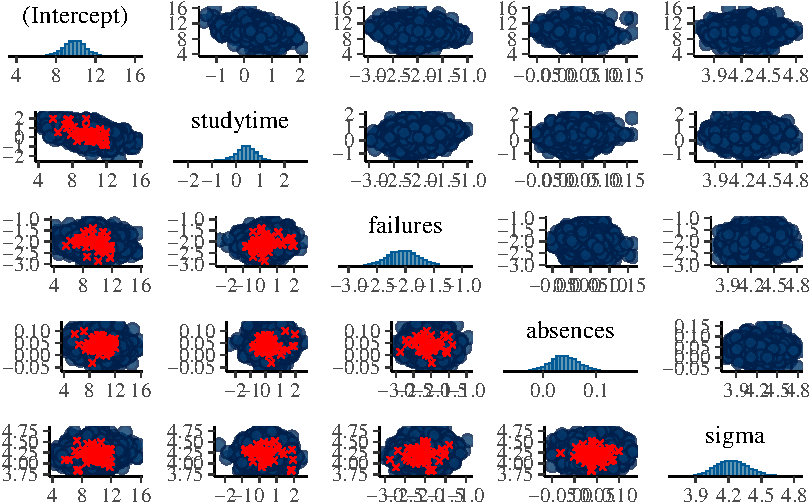
\includegraphics{551-HW-Q2_files/figure-pdf/unnamed-chunk-5-1.pdf}

\begin{Shaded}
\begin{Highlighting}[]
\NormalTok{posterior }\OtherTok{\textless{}{-}} \FunctionTok{as.array}\NormalTok{(fit\_t4)}
\FunctionTok{mcmc\_trace}\NormalTok{(posterior, }\AttributeTok{pars =} \FunctionTok{c}\NormalTok{(}\StringTok{"beta[1]"}\NormalTok{, }\StringTok{"beta[2]"}\NormalTok{, }\StringTok{"sigma"}\NormalTok{))}
\end{Highlighting}
\end{Shaded}

\includegraphics{551-HW-Q2_files/figure-pdf/unnamed-chunk-6-1.pdf}

\begin{Shaded}
\begin{Highlighting}[]
\FunctionTok{library}\NormalTok{(glmnet)}
\end{Highlighting}
\end{Shaded}

\begin{verbatim}
Loading required package: Matrix
\end{verbatim}

\begin{verbatim}
Loaded glmnet 4.1-8
\end{verbatim}

\begin{Shaded}
\begin{Highlighting}[]
\CommentTok{\# Simulated example dataset}
\FunctionTok{set.seed}\NormalTok{(}\DecValTok{123}\NormalTok{)}
\NormalTok{n }\OtherTok{\textless{}{-}} \DecValTok{100}
\NormalTok{data }\OtherTok{\textless{}{-}} \FunctionTok{data.frame}\NormalTok{(}
  \AttributeTok{ratio =} \FunctionTok{rnorm}\NormalTok{(n, }\DecValTok{1300}\NormalTok{, }\DecValTok{100}\NormalTok{),}
  \AttributeTok{contact =} \FunctionTok{runif}\NormalTok{(n, }\DecValTok{5}\NormalTok{, }\DecValTok{23}\NormalTok{),}
  \AttributeTok{conversion =} \FunctionTok{rnorm}\NormalTok{(n, }\FloatTok{0.03}\NormalTok{, }\FloatTok{0.01}\NormalTok{),}
  \AttributeTok{y =} \FunctionTok{rnorm}\NormalTok{(n, }\DecValTok{40}\NormalTok{, }\DecValTok{10}\NormalTok{)}
\NormalTok{)}

\CommentTok{\# Add interaction and squared terms}
\NormalTok{data}\SpecialCharTok{$}\NormalTok{ratio\_sq }\OtherTok{\textless{}{-}}\NormalTok{ data}\SpecialCharTok{$}\NormalTok{ratio}\SpecialCharTok{\^{}}\DecValTok{2}
\NormalTok{data}\SpecialCharTok{$}\NormalTok{contact\_sq }\OtherTok{\textless{}{-}}\NormalTok{ data}\SpecialCharTok{$}\NormalTok{contact}\SpecialCharTok{\^{}}\DecValTok{2}
\NormalTok{data}\SpecialCharTok{$}\NormalTok{conversion\_sq }\OtherTok{\textless{}{-}}\NormalTok{ data}\SpecialCharTok{$}\NormalTok{conversion}\SpecialCharTok{\^{}}\DecValTok{2}
\NormalTok{data}\SpecialCharTok{$}\NormalTok{ratiocontact }\OtherTok{\textless{}{-}}\NormalTok{ data}\SpecialCharTok{$}\NormalTok{ratio }\SpecialCharTok{*}\NormalTok{ data}\SpecialCharTok{$}\NormalTok{contact}
\NormalTok{data}\SpecialCharTok{$}\NormalTok{contactconversion }\OtherTok{\textless{}{-}}\NormalTok{ data}\SpecialCharTok{$}\NormalTok{contact }\SpecialCharTok{*}\NormalTok{ data}\SpecialCharTok{$}\NormalTok{conversion}
\NormalTok{data}\SpecialCharTok{$}\NormalTok{ratioconversion }\OtherTok{\textless{}{-}}\NormalTok{ data}\SpecialCharTok{$}\NormalTok{ratio }\SpecialCharTok{*}\NormalTok{ data}\SpecialCharTok{$}\NormalTok{conversion}

\CommentTok{\# Prepare matrix for glmnet}
\NormalTok{X }\OtherTok{\textless{}{-}} \FunctionTok{as.matrix}\NormalTok{(data[, }\FunctionTok{c}\NormalTok{(}\StringTok{"ratio"}\NormalTok{, }\StringTok{"contact"}\NormalTok{, }\StringTok{"conversion"}\NormalTok{, }\StringTok{"ratio\_sq"}\NormalTok{, }\StringTok{"contact\_sq"}\NormalTok{,}
                        \StringTok{"conversion\_sq"}\NormalTok{, }\StringTok{"ratiocontact"}\NormalTok{, }\StringTok{"contactconversion"}\NormalTok{,}
                        \StringTok{"ratioconversion"}\NormalTok{)])}
\NormalTok{y }\OtherTok{\textless{}{-}}\NormalTok{ data}\SpecialCharTok{$}\NormalTok{y}

\CommentTok{\# Fit ridge regression}
\NormalTok{ridge\_model }\OtherTok{\textless{}{-}} \FunctionTok{glmnet}\NormalTok{(X, y, }\AttributeTok{alpha =} \DecValTok{0}\NormalTok{)  }\CommentTok{\# alpha = 0 for ridge regression}
\NormalTok{ridge\_cv }\OtherTok{\textless{}{-}} \FunctionTok{cv.glmnet}\NormalTok{(X, y, }\AttributeTok{alpha =} \DecValTok{0}\NormalTok{)  }\CommentTok{\# Cross{-}validation to find best lambda}
\NormalTok{ridge\_best\_lambda }\OtherTok{\textless{}{-}}\NormalTok{ ridge\_cv}\SpecialCharTok{$}\NormalTok{lambda.min}

\CommentTok{\# Extract coefficients at best lambda}
\NormalTok{ridge\_coefficients }\OtherTok{\textless{}{-}} \FunctionTok{coef}\NormalTok{(ridge\_cv, }\AttributeTok{s =}\NormalTok{ ridge\_best\_lambda)}
\FunctionTok{print}\NormalTok{(ridge\_coefficients)}
\end{Highlighting}
\end{Shaded}

\begin{verbatim}
10 x 1 sparse Matrix of class "dgCMatrix"
                             s1
(Intercept)        4.125752e+01
ratio              5.145622e-39
contact           -3.678847e-38
conversion         5.997559e-35
ratio_sq           1.828757e-42
contact_sq        -4.366979e-40
conversion_sq      6.464200e-34
ratiocontact      -3.078151e-42
contactconversion  9.398377e-37
ratioconversion    5.034607e-38
\end{verbatim}

\begin{Shaded}
\begin{Highlighting}[]
\CommentTok{\# install.packages("brms")}
\FunctionTok{library}\NormalTok{(brms)}
\end{Highlighting}
\end{Shaded}

\begin{verbatim}
Loading required package: Rcpp
\end{verbatim}

\begin{verbatim}
Loading 'brms' package (version 2.22.0). Useful instructions
can be found by typing help('brms'). A more detailed introduction
to the package is available through vignette('brms_overview').
\end{verbatim}

\begin{verbatim}

Attaching package: 'brms'
\end{verbatim}

\begin{verbatim}
The following object is masked from 'package:bayesplot':

    rhat
\end{verbatim}

\begin{verbatim}
The following objects are masked from 'package:MCMCpack':

    ddirichlet, rdirichlet
\end{verbatim}

\begin{verbatim}
The following object is masked from 'package:rstan':

    loo
\end{verbatim}

\begin{verbatim}
The following object is masked from 'package:stats':

    ar
\end{verbatim}

\begin{Shaded}
\begin{Highlighting}[]
\CommentTok{\# Fitting a Bayesian regression model}
\NormalTok{posterior\_model }\OtherTok{\textless{}{-}} \FunctionTok{brm}\NormalTok{(}
\NormalTok{  y }\SpecialCharTok{\textasciitilde{}}\NormalTok{ ratio }\SpecialCharTok{+}\NormalTok{ contact }\SpecialCharTok{+}\NormalTok{ conversion }\SpecialCharTok{+}\NormalTok{ ratio\_sq }\SpecialCharTok{+}\NormalTok{ contact\_sq }\SpecialCharTok{+}\NormalTok{ conversion\_sq }\SpecialCharTok{+}
\NormalTok{    ratiocontact }\SpecialCharTok{+}\NormalTok{ contactconversion }\SpecialCharTok{+}\NormalTok{ ratioconversion,}
  \AttributeTok{data =}\NormalTok{ data,}
  \AttributeTok{family =} \FunctionTok{gaussian}\NormalTok{()}
\NormalTok{)}
\end{Highlighting}
\end{Shaded}

\begin{verbatim}
Compiling Stan program...
\end{verbatim}

\begin{verbatim}
Start sampling
\end{verbatim}

\begin{verbatim}

SAMPLING FOR MODEL 'anon_model' NOW (CHAIN 1).
Chain 1: 
Chain 1: Gradient evaluation took 5.9e-05 seconds
Chain 1: 1000 transitions using 10 leapfrog steps per transition would take 0.59 seconds.
Chain 1: Adjust your expectations accordingly!
Chain 1: 
Chain 1: 
Chain 1: Iteration:    1 / 2000 [  0%]  (Warmup)
Chain 1: Iteration:  200 / 2000 [ 10%]  (Warmup)
Chain 1: Iteration:  400 / 2000 [ 20%]  (Warmup)
Chain 1: Iteration:  600 / 2000 [ 30%]  (Warmup)
Chain 1: Iteration:  800 / 2000 [ 40%]  (Warmup)
Chain 1: Iteration: 1000 / 2000 [ 50%]  (Warmup)
Chain 1: Iteration: 1001 / 2000 [ 50%]  (Sampling)
Chain 1: Iteration: 1200 / 2000 [ 60%]  (Sampling)
Chain 1: Iteration: 1400 / 2000 [ 70%]  (Sampling)
Chain 1: Iteration: 1600 / 2000 [ 80%]  (Sampling)
Chain 1: Iteration: 1800 / 2000 [ 90%]  (Sampling)
Chain 1: Iteration: 2000 / 2000 [100%]  (Sampling)
Chain 1: 
Chain 1:  Elapsed Time: 3.279 seconds (Warm-up)
Chain 1:                1.005 seconds (Sampling)
Chain 1:                4.284 seconds (Total)
Chain 1: 

SAMPLING FOR MODEL 'anon_model' NOW (CHAIN 2).
Chain 2: 
Chain 2: Gradient evaluation took 9e-06 seconds
Chain 2: 1000 transitions using 10 leapfrog steps per transition would take 0.09 seconds.
Chain 2: Adjust your expectations accordingly!
Chain 2: 
Chain 2: 
Chain 2: Iteration:    1 / 2000 [  0%]  (Warmup)
Chain 2: Iteration:  200 / 2000 [ 10%]  (Warmup)
Chain 2: Iteration:  400 / 2000 [ 20%]  (Warmup)
Chain 2: Iteration:  600 / 2000 [ 30%]  (Warmup)
Chain 2: Iteration:  800 / 2000 [ 40%]  (Warmup)
Chain 2: Iteration: 1000 / 2000 [ 50%]  (Warmup)
Chain 2: Iteration: 1001 / 2000 [ 50%]  (Sampling)
Chain 2: Iteration: 1200 / 2000 [ 60%]  (Sampling)
Chain 2: Iteration: 1400 / 2000 [ 70%]  (Sampling)
Chain 2: Iteration: 1600 / 2000 [ 80%]  (Sampling)
Chain 2: Iteration: 1800 / 2000 [ 90%]  (Sampling)
Chain 2: Iteration: 2000 / 2000 [100%]  (Sampling)
Chain 2: 
Chain 2:  Elapsed Time: 0.29 seconds (Warm-up)
Chain 2:                5.532 seconds (Sampling)
Chain 2:                5.822 seconds (Total)
Chain 2: 

SAMPLING FOR MODEL 'anon_model' NOW (CHAIN 3).
Chain 3: 
Chain 3: Gradient evaluation took 4e-05 seconds
Chain 3: 1000 transitions using 10 leapfrog steps per transition would take 0.4 seconds.
Chain 3: Adjust your expectations accordingly!
Chain 3: 
Chain 3: 
Chain 3: Iteration:    1 / 2000 [  0%]  (Warmup)
Chain 3: Iteration:  200 / 2000 [ 10%]  (Warmup)
Chain 3: Iteration:  400 / 2000 [ 20%]  (Warmup)
Chain 3: Iteration:  600 / 2000 [ 30%]  (Warmup)
Chain 3: Iteration:  800 / 2000 [ 40%]  (Warmup)
Chain 3: Iteration: 1000 / 2000 [ 50%]  (Warmup)
Chain 3: Iteration: 1001 / 2000 [ 50%]  (Sampling)
Chain 3: Iteration: 1200 / 2000 [ 60%]  (Sampling)
Chain 3: Iteration: 1400 / 2000 [ 70%]  (Sampling)
Chain 3: Iteration: 1600 / 2000 [ 80%]  (Sampling)
Chain 3: Iteration: 1800 / 2000 [ 90%]  (Sampling)
Chain 3: Iteration: 2000 / 2000 [100%]  (Sampling)
Chain 3: 
Chain 3:  Elapsed Time: 2.928 seconds (Warm-up)
Chain 3:                2.214 seconds (Sampling)
Chain 3:                5.142 seconds (Total)
Chain 3: 

SAMPLING FOR MODEL 'anon_model' NOW (CHAIN 4).
Chain 4: 
Chain 4: Gradient evaluation took 6.1e-05 seconds
Chain 4: 1000 transitions using 10 leapfrog steps per transition would take 0.61 seconds.
Chain 4: Adjust your expectations accordingly!
Chain 4: 
Chain 4: 
Chain 4: Iteration:    1 / 2000 [  0%]  (Warmup)
Chain 4: Iteration:  200 / 2000 [ 10%]  (Warmup)
Chain 4: Iteration:  400 / 2000 [ 20%]  (Warmup)
Chain 4: Iteration:  600 / 2000 [ 30%]  (Warmup)
Chain 4: Iteration:  800 / 2000 [ 40%]  (Warmup)
Chain 4: Iteration: 1000 / 2000 [ 50%]  (Warmup)
Chain 4: Iteration: 1001 / 2000 [ 50%]  (Sampling)
Chain 4: Iteration: 1200 / 2000 [ 60%]  (Sampling)
Chain 4: Iteration: 1400 / 2000 [ 70%]  (Sampling)
Chain 4: Iteration: 1600 / 2000 [ 80%]  (Sampling)
Chain 4: Iteration: 1800 / 2000 [ 90%]  (Sampling)
Chain 4: Iteration: 2000 / 2000 [100%]  (Sampling)
Chain 4: 
Chain 4:  Elapsed Time: 3.514 seconds (Warm-up)
Chain 4:                5.579 seconds (Sampling)
Chain 4:                9.093 seconds (Total)
Chain 4: 
\end{verbatim}

\begin{verbatim}
Warning: There were 1352 divergent transitions after warmup. See
https://mc-stan.org/misc/warnings.html#divergent-transitions-after-warmup
to find out why this is a problem and how to eliminate them.
\end{verbatim}

\begin{verbatim}
Warning: There were 2371 transitions after warmup that exceeded the maximum treedepth. Increase max_treedepth above 10. See
https://mc-stan.org/misc/warnings.html#maximum-treedepth-exceeded
\end{verbatim}

\begin{verbatim}
Warning: There were 3 chains where the estimated Bayesian Fraction of Missing Information was low. See
https://mc-stan.org/misc/warnings.html#bfmi-low
\end{verbatim}

\begin{verbatim}
Warning: Examine the pairs() plot to diagnose sampling problems
\end{verbatim}

\begin{verbatim}
Warning: The largest R-hat is 3.07, indicating chains have not mixed.
Running the chains for more iterations may help. See
https://mc-stan.org/misc/warnings.html#r-hat
\end{verbatim}

\begin{verbatim}
Warning: Bulk Effective Samples Size (ESS) is too low, indicating posterior means and medians may be unreliable.
Running the chains for more iterations may help. See
https://mc-stan.org/misc/warnings.html#bulk-ess
\end{verbatim}

\begin{verbatim}
Warning: Tail Effective Samples Size (ESS) is too low, indicating posterior variances and tail quantiles may be unreliable.
Running the chains for more iterations may help. See
https://mc-stan.org/misc/warnings.html#tail-ess
\end{verbatim}

\begin{Shaded}
\begin{Highlighting}[]
\CommentTok{\# Converting to array }
\NormalTok{posterior\_array }\OtherTok{\textless{}{-}} \FunctionTok{as.array}\NormalTok{(posterior\_model)}

\CommentTok{\# inspecting posterior samples}
\FunctionTok{summary}\NormalTok{(posterior\_array) }
\end{Highlighting}
\end{Shaded}

\begin{verbatim}
     Min.   1st Qu.    Median      Mean   3rd Qu.      Max. 
-4707.337    -1.865     0.000   -16.086     1.579  2590.786 
\end{verbatim}

\begin{Shaded}
\begin{Highlighting}[]
\CommentTok{\# Fit LASSO regression}
\NormalTok{lasso\_model }\OtherTok{\textless{}{-}} \FunctionTok{glmnet}\NormalTok{(X, y, }\AttributeTok{alpha =} \DecValTok{1}\NormalTok{)  }\CommentTok{\# alpha = 1 for LASSO}
\NormalTok{lasso\_cv }\OtherTok{\textless{}{-}} \FunctionTok{cv.glmnet}\NormalTok{(X, y, }\AttributeTok{alpha =} \DecValTok{1}\NormalTok{)  }\CommentTok{\# Cross{-}validation to select lambda}
\NormalTok{lasso\_best\_lambda }\OtherTok{\textless{}{-}}\NormalTok{ lasso\_cv}\SpecialCharTok{$}\NormalTok{lambda.min}
\NormalTok{lasso\_coefficients }\OtherTok{\textless{}{-}} \FunctionTok{coef}\NormalTok{(lasso\_cv, }\AttributeTok{s =}\NormalTok{ lasso\_best\_lambda)}
\NormalTok{lasso\_coefficients}
\end{Highlighting}
\end{Shaded}

\begin{verbatim}
10 x 1 sparse Matrix of class "dgCMatrix"
                        s1
(Intercept)       41.25752
ratio              .      
contact            .      
conversion         .      
ratio_sq           .      
contact_sq         .      
conversion_sq      .      
ratiocontact       .      
contactconversion  .      
ratioconversion    .      
\end{verbatim}

\begin{Shaded}
\begin{Highlighting}[]
\CommentTok{\# install.packages("kernlab")}
\FunctionTok{library}\NormalTok{(kernlab)}
\end{Highlighting}
\end{Shaded}

\begin{verbatim}

Attaching package: 'kernlab'
\end{verbatim}

\begin{verbatim}
The following object is masked from 'package:brms':

    prior
\end{verbatim}

\begin{verbatim}
The following object is masked from 'package:coda':

    nvar
\end{verbatim}

\begin{Shaded}
\begin{Highlighting}[]
\CommentTok{\# Fit Gaussian Process model}
\NormalTok{gpr\_model }\OtherTok{\textless{}{-}} \FunctionTok{gausspr}\NormalTok{(X, y, }\AttributeTok{kernel =} \StringTok{"rbfdot"}\NormalTok{)}
\end{Highlighting}
\end{Shaded}

\begin{verbatim}
Using automatic sigma estimation (sigest) for RBF or laplace kernel 
\end{verbatim}

\begin{Shaded}
\begin{Highlighting}[]
\NormalTok{gpr\_predictions }\OtherTok{\textless{}{-}} \FunctionTok{predict}\NormalTok{(gpr\_model, X)}

\CommentTok{\# Compare predicted and observed values}
\NormalTok{pred\_obs }\OtherTok{\textless{}{-}} \FunctionTok{data.frame}\NormalTok{(}\AttributeTok{Observed =}\NormalTok{ y, }\AttributeTok{Predicted =}\NormalTok{ gpr\_predictions)}
\FunctionTok{print}\NormalTok{ (pred\_obs)}
\end{Highlighting}
\end{Shaded}

\begin{verbatim}
    Observed Predicted
1   36.24397  44.74188
2   34.38124  39.78353
3   36.56083  41.75616
4   40.90497  37.03168
5   55.98509  41.44438
6   39.11435  41.86310
7   50.80799  41.34531
8   46.30754  39.60757
9   38.86360  45.10099
10  24.67098  41.37619
11  34.78883  40.13050
12  35.10130  39.52646
13  40.47154  40.21119
14  53.00199  46.88429
15  62.93079  43.27939
16  55.47581  42.68169
17  38.66849  41.01601
18  22.43473  36.76778
19  36.11220  45.06391
20  40.89207  43.29422
21  48.45013  41.23122
22  49.62528  45.42798
23  46.84309  43.19674
24  26.04726  36.11094
25  48.49643  41.56906
26  35.53443  34.04549
27  41.74803  41.60458
28  40.74551  44.89281
29  44.28167  42.65687
30  40.24675  42.53565
31  23.32525  38.19324
32  47.36496  42.85880
33  43.86027  41.73808
34  37.34348  42.70020
35  41.18145  39.47314
36  41.34039  40.55450
37  42.21019  39.69249
38  56.40846  46.72785
39  37.80950  44.14394
40  41.68065  43.12449
41  51.68384  44.63494
42  50.54181  43.63918
43  51.45263  44.31106
44  34.22532  40.73541
45  60.02483  43.55182
46  40.66701  34.01140
47  58.66852  44.55460
48  26.49097  36.87696
49  40.20984  42.84938
50  52.49915  37.61271
51  32.84758  40.91816
52  32.47311  42.71082
53  30.61461  43.19264
54  29.47487  35.26460
55  35.62840  41.04758
56  43.31179  41.48455
57  19.85790  37.11911
58  42.11980  39.91510
59  52.36675  42.00927
60  60.37574  47.06590
61  53.01176  46.77845
62  47.56775  44.32374
63  22.73270  38.71778
64  33.98493  39.79466
65  36.47954  35.89748
66  47.03524  41.70508
67  38.94329  39.87598
68  27.41351  38.30541
69  56.84436  44.19056
70  49.11391  43.42324
71  42.37430  42.12762
72  52.18109  46.26578
73  26.61226  36.70861
74  46.60820  45.48736
75  34.77088  43.01431
76  46.83746  44.94613
77  39.39178  41.19710
78  46.32961  36.97452
79  53.35518  41.83494
80  40.07290  37.86481
81  50.17559  38.53684
82  28.11566  40.35601
83  32.78396  43.71509
84  55.19218  40.72602
85  43.77388  42.41952
86  19.47777  37.40476
87  26.35963  38.13627
88  37.99219  39.89370
89  48.65779  44.64967
90  38.98117  40.66686
91  46.24187  41.46462
92  49.59005  41.10951
93  56.71055  42.09712
94  40.56017  37.64849
95  39.48018  43.25426
96  22.46763  33.94102
97  40.99328  41.26592
98  34.28150  44.88015
99  30.25990  41.39171
100 38.20094  41.47033
\end{verbatim}

\begin{Shaded}
\begin{Highlighting}[]
\CommentTok{\# colnames(pred\_obs)}
\end{Highlighting}
\end{Shaded}

\begin{Shaded}
\begin{Highlighting}[]
\CommentTok{\# Error metrics}
\NormalTok{mse }\OtherTok{\textless{}{-}} \FunctionTok{mean}\NormalTok{((pred\_obs}\SpecialCharTok{$}\NormalTok{Observed }\SpecialCharTok{{-}}\NormalTok{ pred\_obs}\SpecialCharTok{$}\NormalTok{Predicted)}\SpecialCharTok{\^{}}\DecValTok{2}\NormalTok{)}
\NormalTok{rmse }\OtherTok{\textless{}{-}} \FunctionTok{sqrt}\NormalTok{(mse)}
\NormalTok{mae }\OtherTok{\textless{}{-}} \FunctionTok{mean}\NormalTok{(}\FunctionTok{abs}\NormalTok{(pred\_obs}\SpecialCharTok{$}\NormalTok{Observed }\SpecialCharTok{{-}}\NormalTok{ pred\_obs}\SpecialCharTok{$}\NormalTok{Predicted))}
\NormalTok{r\_squared }\OtherTok{\textless{}{-}} \DecValTok{1} \SpecialCharTok{{-}}\NormalTok{ (}\FunctionTok{sum}\NormalTok{((pred\_obs}\SpecialCharTok{$}\NormalTok{Observed }\SpecialCharTok{{-}}\NormalTok{ pred\_obs}\SpecialCharTok{$}\NormalTok{Predicted)}\SpecialCharTok{\^{}}\DecValTok{2}\NormalTok{) }\SpecialCharTok{/} 
                    \FunctionTok{sum}\NormalTok{((pred\_obs}\SpecialCharTok{$}\NormalTok{Observed }\SpecialCharTok{{-}} \FunctionTok{mean}\NormalTok{(pred\_obs}\SpecialCharTok{$}\NormalTok{Observed))}\SpecialCharTok{\^{}}\DecValTok{2}\NormalTok{))}

\FunctionTok{cat}\NormalTok{(}\StringTok{"MSE:"}\NormalTok{, mse, }\StringTok{"}\SpecialCharTok{\textbackslash{}n}\StringTok{RMSE:"}\NormalTok{, rmse, }\StringTok{"}\SpecialCharTok{\textbackslash{}n}\StringTok{MAE:"}\NormalTok{, mae, }\StringTok{"}\SpecialCharTok{\textbackslash{}n}\StringTok{R{-}squared:"}\NormalTok{, r\_squared)}
\end{Highlighting}
\end{Shaded}

\begin{verbatim}
MSE: 73.76403 
RMSE: 8.588599 
MAE: 7.058613 
R-squared: 0.2422157
\end{verbatim}

\begin{Shaded}
\begin{Highlighting}[]
\CommentTok{\# Visualization}
\FunctionTok{library}\NormalTok{(ggplot2)}
\end{Highlighting}
\end{Shaded}

\begin{verbatim}

Attaching package: 'ggplot2'
\end{verbatim}

\begin{verbatim}
The following object is masked from 'package:kernlab':

    alpha
\end{verbatim}

\begin{Shaded}
\begin{Highlighting}[]
\FunctionTok{ggplot}\NormalTok{(pred\_obs, }\FunctionTok{aes}\NormalTok{(}\AttributeTok{x =}\NormalTok{ Observed, }\AttributeTok{y =}\NormalTok{ Predicted)) }\SpecialCharTok{+}
  \FunctionTok{geom\_point}\NormalTok{(}\AttributeTok{color =} \StringTok{"blue"}\NormalTok{, }\AttributeTok{size =} \FloatTok{2.5}\NormalTok{) }\SpecialCharTok{+}
  \FunctionTok{geom\_abline}\NormalTok{(}\AttributeTok{intercept =} \DecValTok{0}\NormalTok{, }\AttributeTok{slope =} \DecValTok{1}\NormalTok{, }\AttributeTok{color =} \StringTok{"red"}\NormalTok{, }\AttributeTok{linetype =} \StringTok{"dashed"}\NormalTok{) }\SpecialCharTok{+}
  \FunctionTok{labs}\NormalTok{(}\AttributeTok{title =} \StringTok{"Observed vs Predicted Values"}\NormalTok{, }\AttributeTok{x =} \StringTok{"Observed"}\NormalTok{, }\AttributeTok{y =} \StringTok{"Predicted"}\NormalTok{) }\SpecialCharTok{+}
  \FunctionTok{theme\_minimal}\NormalTok{()}
\end{Highlighting}
\end{Shaded}

\includegraphics{551-HW-Q2_files/figure-pdf/unnamed-chunk-12-1.pdf}

\begin{Shaded}
\begin{Highlighting}[]
\CommentTok{\# Residuals}
\NormalTok{pred\_obs}\SpecialCharTok{$}\NormalTok{Residuals }\OtherTok{\textless{}{-}}\NormalTok{ pred\_obs}\SpecialCharTok{$}\NormalTok{Observed }\SpecialCharTok{{-}}\NormalTok{ pred\_obs}\SpecialCharTok{$}\NormalTok{Predicted}

\CommentTok{\# Plot residuals}
\FunctionTok{ggplot}\NormalTok{(pred\_obs, }\FunctionTok{aes}\NormalTok{(}\AttributeTok{x =}\NormalTok{ Observed, }\AttributeTok{y =}\NormalTok{ Residuals)) }\SpecialCharTok{+}
  \FunctionTok{geom\_point}\NormalTok{(}\AttributeTok{color =} \StringTok{"purple"}\NormalTok{, }\AttributeTok{size =} \FloatTok{2.5}\NormalTok{) }\SpecialCharTok{+}
  \FunctionTok{geom\_hline}\NormalTok{(}\AttributeTok{yintercept =} \DecValTok{0}\NormalTok{, }\AttributeTok{color =} \StringTok{"red"}\NormalTok{, }\AttributeTok{linetype =} \StringTok{"dashed"}\NormalTok{) }\SpecialCharTok{+}
  \FunctionTok{labs}\NormalTok{(}\AttributeTok{title =} \StringTok{"Residuals vs Observed Values"}\NormalTok{, }\AttributeTok{x =} \StringTok{"Observed"}\NormalTok{, }\AttributeTok{y =} \StringTok{"Residuals"}\NormalTok{) }\SpecialCharTok{+}
  \FunctionTok{theme\_minimal}\NormalTok{()}
\end{Highlighting}
\end{Shaded}

\includegraphics{551-HW-Q2_files/figure-pdf/unnamed-chunk-13-1.pdf}




\end{document}
